% Options for packages loaded elsewhere
\PassOptionsToPackage{unicode}{hyperref}
\PassOptionsToPackage{hyphens}{url}
%
\documentclass[
]{article}
\usepackage{amsmath,amssymb}
\usepackage{lmodern}
\usepackage{iftex}
\ifPDFTeX
  \usepackage[T1]{fontenc}
  \usepackage[utf8]{inputenc}
  \usepackage{textcomp} % provide euro and other symbols
\else % if luatex or xetex
  \usepackage{unicode-math}
  \defaultfontfeatures{Scale=MatchLowercase}
  \defaultfontfeatures[\rmfamily]{Ligatures=TeX,Scale=1}
\fi
% Use upquote if available, for straight quotes in verbatim environments
\IfFileExists{upquote.sty}{\usepackage{upquote}}{}
\IfFileExists{microtype.sty}{% use microtype if available
  \usepackage[]{microtype}
  \UseMicrotypeSet[protrusion]{basicmath} % disable protrusion for tt fonts
}{}
\makeatletter
\@ifundefined{KOMAClassName}{% if non-KOMA class
  \IfFileExists{parskip.sty}{%
    \usepackage{parskip}
  }{% else
    \setlength{\parindent}{0pt}
    \setlength{\parskip}{6pt plus 2pt minus 1pt}}
}{% if KOMA class
  \KOMAoptions{parskip=half}}
\makeatother
\usepackage{xcolor}
\IfFileExists{xurl.sty}{\usepackage{xurl}}{} % add URL line breaks if available
\IfFileExists{bookmark.sty}{\usepackage{bookmark}}{\usepackage{hyperref}}
\hypersetup{
  pdftitle={Data Analysis Coursebook},
  pdfauthor={Marcell Granat \& Zoltan Madari},
  hidelinks,
  pdfcreator={LaTeX via pandoc}}
\urlstyle{same} % disable monospaced font for URLs
\usepackage[margin=1in]{geometry}
\usepackage{longtable,booktabs,array}
\usepackage{calc} % for calculating minipage widths
% Correct order of tables after \paragraph or \subparagraph
\usepackage{etoolbox}
\makeatletter
\patchcmd\longtable{\par}{\if@noskipsec\mbox{}\fi\par}{}{}
\makeatother
% Allow footnotes in longtable head/foot
\IfFileExists{footnotehyper.sty}{\usepackage{footnotehyper}}{\usepackage{footnote}}
\makesavenoteenv{longtable}
\usepackage{graphicx}
\makeatletter
\def\maxwidth{\ifdim\Gin@nat@width>\linewidth\linewidth\else\Gin@nat@width\fi}
\def\maxheight{\ifdim\Gin@nat@height>\textheight\textheight\else\Gin@nat@height\fi}
\makeatother
% Scale images if necessary, so that they will not overflow the page
% margins by default, and it is still possible to overwrite the defaults
% using explicit options in \includegraphics[width, height, ...]{}
\setkeys{Gin}{width=\maxwidth,height=\maxheight,keepaspectratio}
% Set default figure placement to htbp
\makeatletter
\def\fps@figure{htbp}
\makeatother
\setlength{\emergencystretch}{3em} % prevent overfull lines
\providecommand{\tightlist}{%
  \setlength{\itemsep}{0pt}\setlength{\parskip}{0pt}}
\setcounter{secnumdepth}{5}
\usepackage{pdfpages}

\usepackage{booktabs}
\usepackage{amsthm}
\makeatletter
\def\thm@space@setup{%
  \thm@preskip=8pt plus 2pt minus 4pt
  \thm@postskip=\thm@preskip
}
\makeatother


% sidebar environment
\usepackage{framed,color}
\definecolor{shadecolor}{RGB}{242,242,242}
\makeatletter
\newenvironment{sidebar}{%
\medskip{}
\setlength{\fboxsep}{.8em}
 \def\at@end@of@kframe{}%
 \ifinner\ifhmode%
  \def\at@end@of@kframe{\end{minipage}}%
  \begin{minipage}{\columnwidth}%
 \fi\fi%
 \def\FrameCommand##1{\hskip\@totalleftmargin \hskip-\fboxsep
 \colorbox{shadecolor}{##1}\hskip-\fboxsep
     % There is no \\@totalrightmargin, so:
     \hskip-\linewidth \hskip-\@totalleftmargin \hskip\columnwidth}%
 \MakeFramed {\advance\hsize-\width
   \@totalleftmargin\z@ \linewidth\hsize
   \@setminipage}}%
 {\par\unskip\endMakeFramed%
 \at@end@of@kframe}
\makeatother
\ifLuaTeX
  \usepackage{selnolig}  % disable illegal ligatures
\fi
\usepackage[]{natbib}
\bibliographystyle{plainnat}

\title{\textbf{Data Analysis} Coursebook}
\author{Marcell Granat \& Zoltan Madari}
\date{}

\begin{document}
\maketitle

{
\setcounter{tocdepth}{2}
\tableofcontents
}
\pagebreak

\hypertarget{welcome}{%
\section*{Welcome}\label{welcome}}
\addcontentsline{toc}{section}{Welcome}

\emph{I hope this message finds you well.}

This is an online bookdown file, which we plan to \emph{update regularly} with the class material. We suggest that you to write the code simultaneously with us at seminar, but bugs can always occur out of the blue\ldots{} If you missed something or just want to revisit the topic with additional comments (probably before the exam day) this page is here to help.

At the end of the course you should know:

\begin{itemize}
\item
  What are data types, data quality, and data preprocessing?
\item
  What are the components of \texttt{tidyverse} and what are their advantage?
\item
  What are density, distribution function, quantile functions?
\item
  What are data clustering techniques?
\item
  What are the main techniques for association analysis?
\end{itemize}

We will work with \texttt{R}, one the most loved statistical programming language. Do not be afraid if you do not have any programming experience, this is a beginner course. However, by the end of the program, we hope you will find useful the concept and practical tips we offer, and you will be able to solve your own real life data analysis issues.

\hypertarget{syllabus}{%
\section*{Syllabus}\label{syllabus}}
\addcontentsline{toc}{section}{Syllabus}

\hypertarget{topics}{%
\subsection{Topics}\label{topics}}

\begin{itemize}
\item
  \textbf{Basic R knowledge (Week 1)}

  \begin{itemize}
  \item
    Data categorize, sampling, importing-exporting
  \item
    Types, tables, selection, objects, functions
  \end{itemize}
\item
  \textbf{Data manipulation in Tidyverse (Week 2)}

  \begin{itemize}
  \item
    Filter, group\_by, arrange, summarize commands
  \item
    purr
  \item
    \%\textgreater\%
  \item
    Join (mutating, filtering)
  \item
    tidy data (longer, wider)
  \end{itemize}
\item
  \textbf{Visualization with ggplot2 (Week 3)}

  \begin{itemize}
  \item
    Layers, facets, geoms
  \item
    Descriptive statistics in R
  \item
    Summary statistics, variability, correlation, covariance
  \item
    Extreme values, problem of missing values
  \end{itemize}
\item
  \textbf{Statistical estimation (Week 4)}

  \begin{itemize}
  \tightlist
  \item
    Distributions
  \item
    Sample techniques, confidence intervals, standard error
  \end{itemize}
\item
  \textbf{Hypothesis testing I (Week 5)}

  \begin{itemize}
  \item
    Inductive statistics in R
  \item
    Null and alternative hypothesis, t-test, p-value, fals
    positive/negative, Type I and II error
  \end{itemize}
\item
  \textbf{Hypothesis testing II (Week 6)}

  \begin{itemize}
  \tightlist
  \item
    Relation testing in R
  \end{itemize}
\item
  \textbf{Project presentations (Week 7)}
\end{itemize}

\hypertarget{requirements}{%
\subsection{\texorpdfstring{\textbf{Requirements}}{Requirements}}\label{requirements}}

\begin{itemize}
\item
  \textbf{Test} (30\%): 90 min task solution in R + explanation (exam week)
\item
  \textbf{Project} (25\%): groups (3-4 students), one detailed report
  (essay) and one - \textbf{presentation}
\item
  \textbf{Homeworks} and essays (45\%)
\item
  \textbf{Extra} tasks (+5\%)
\end{itemize}

\hypertarget{project}{%
\subsubsection{Project}\label{project}}

By the end of the course you have to make a statistical report about your own research project in small groups. You have to find a proper dataset (kaggle, eurostat, UCI datasets etc.) or conduct an own survey in optional topic.

At week 7 you will hold a presentation about your findings and results. At the end of the week you will upload your detailed essay about your project work.

\hypertarget{homework}{%
\subsubsection{Homework}\label{homework}}

During the Study period you get 3-5 homeworks. The number of homeworks depends ont he material progress. It could be R code writing or R code writing and analysis (short essay about methods and results).

\begin{longtable}[]{@{}ll@{}}
\caption{Grades}\tabularnewline
\toprule
\endhead
0-50\% & Fail (1) \\
51-62\% & Pass (2) \\
63-74\% & Satisfactory (3) \\
75-86\% & Good (4) \\
87-100\% & excellent (5) \\
\bottomrule
\end{longtable}

\hypertarget{recommended-compulsory-reading}{%
\subsection{Recommended (compulsory) reading}\label{recommended-compulsory-reading}}

\begin{itemize}
\item
  \href{http://r4ds.had.co.nz/}{\textbf{Grolemund G \& Wickham H:
  R for Data Science}}
\item
  Gábor Békés \& Gábor Kézdi: Data Analysis:
  Patterns, Prediction and Causality
\end{itemize}

\hypertarget{part-week-1}{%
\part*{Week 1}\label{part-week-1}}
\addcontentsline{toc}{part}{Week 1}

\hypertarget{lecture1}{%
\section{Lecture 1}\label{lecture1}}

\hypertarget{seminar1}{%
\section{Introduction to R}\label{seminar1}}

\hypertarget{why-r}{%
\subsection{Why R?}\label{why-r}}

In this chapter we will discuss the basics of R programming.
R is a free software, used by millions in the field of statistics, data science, economics and many others.

\href{https://www.facebook.com/Rmemes0/photos/a.1230204967031792/2971372822914989/}{
\includegraphics[width=6.25in,height=\textheight]{images/meme_free.jpg}}

The R programming language is an important tool for data related tasks, but it is much more.
Just like other programming languages, R has many additional packages, which can extend its basic functionality.
R has a great (probably the best) graphical tools to create your charts, and with shiny, you can easily build your minimalist web applications.
We will learn about data manipulation, analysis and how to create awesome reports, like dashboards.

\hypertarget{layout}{%
\subsection{Setup}\label{layout}}

You can download R and RStudio from the official site of \href{https://www.rstudio.com/products/rstudio/download/\#download}{RStudio}.
Please install the appropriate version based on your OS, and do not forget that you also have to install R as well.

\href{https://www.rstudio.com/products/rstudio/download/\#download}{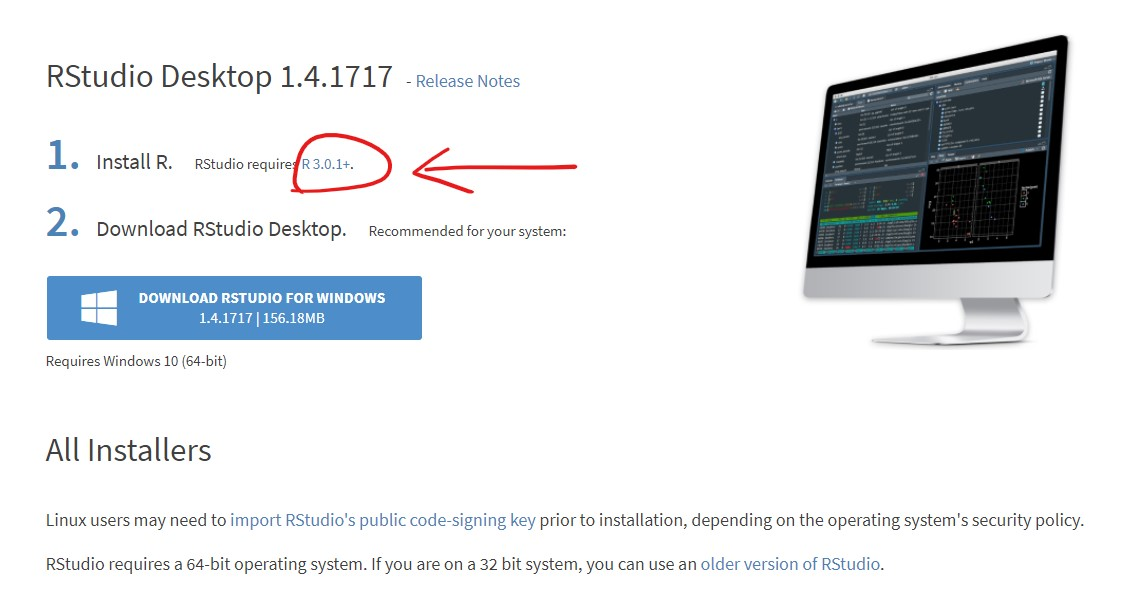
\includegraphics[width=6.25in,height=\textheight]{images/installr.jpg}}

\href{https://cran.rstudio.com/}{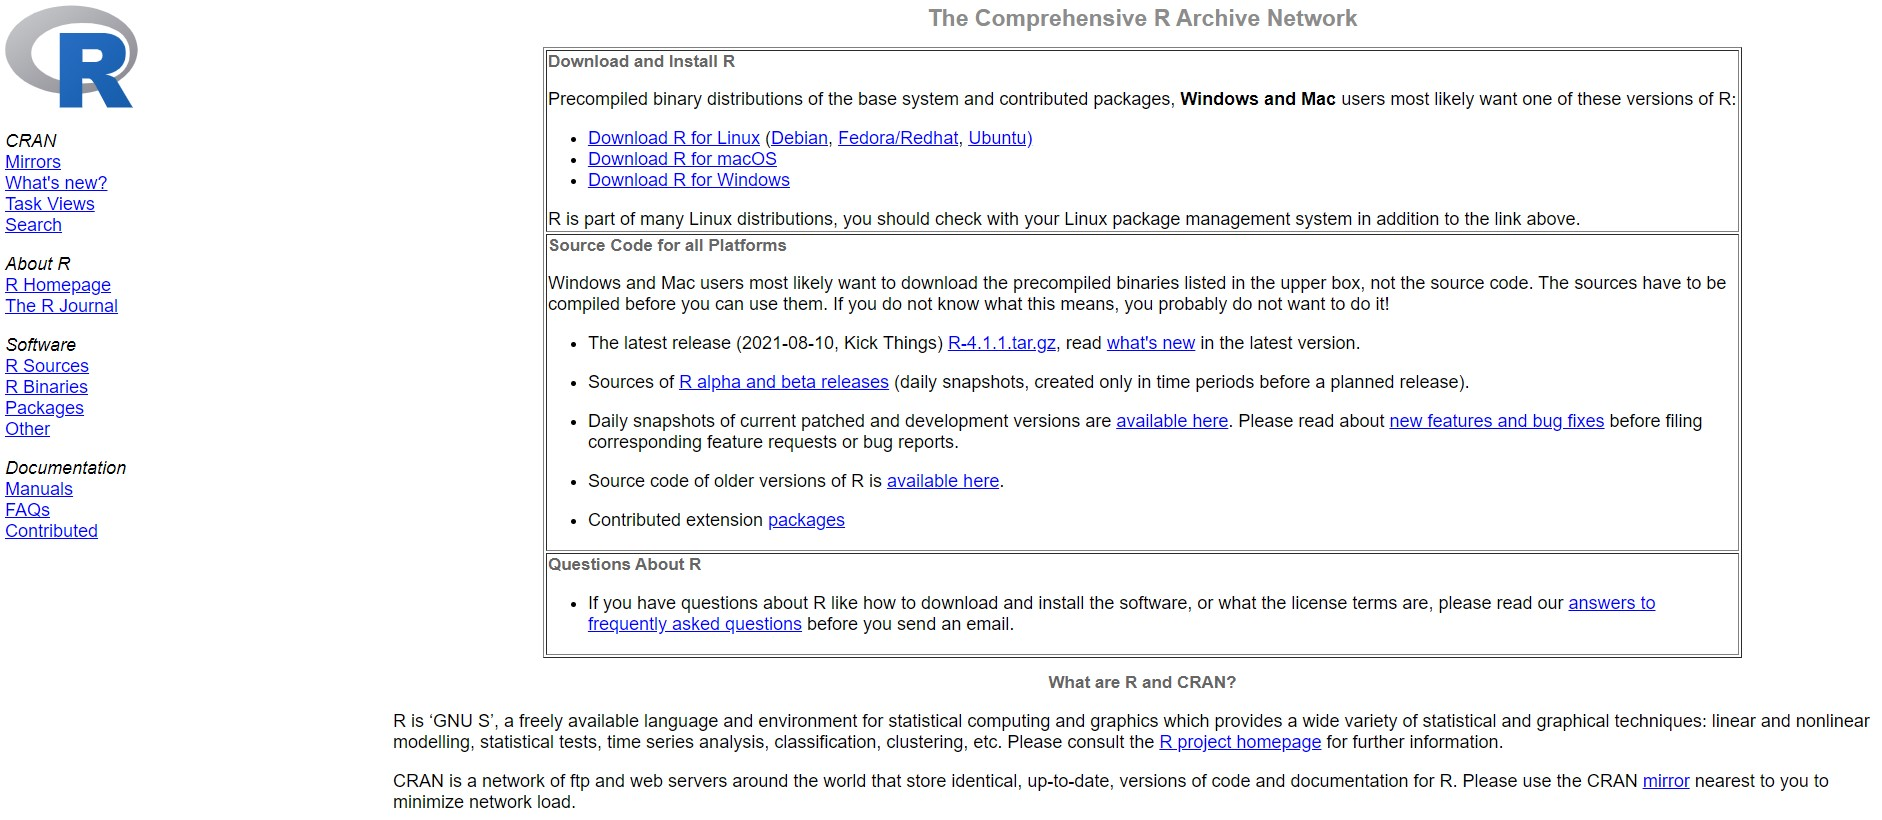
\includegraphics[width=6.25in,height=\textheight]{images/installr2.jpg}}

Run R's installer file after the downloading process is finished.
Next, we will also need the RStudio.

\href{https://www.rstudio.com/products/rstudio/download/\#download}{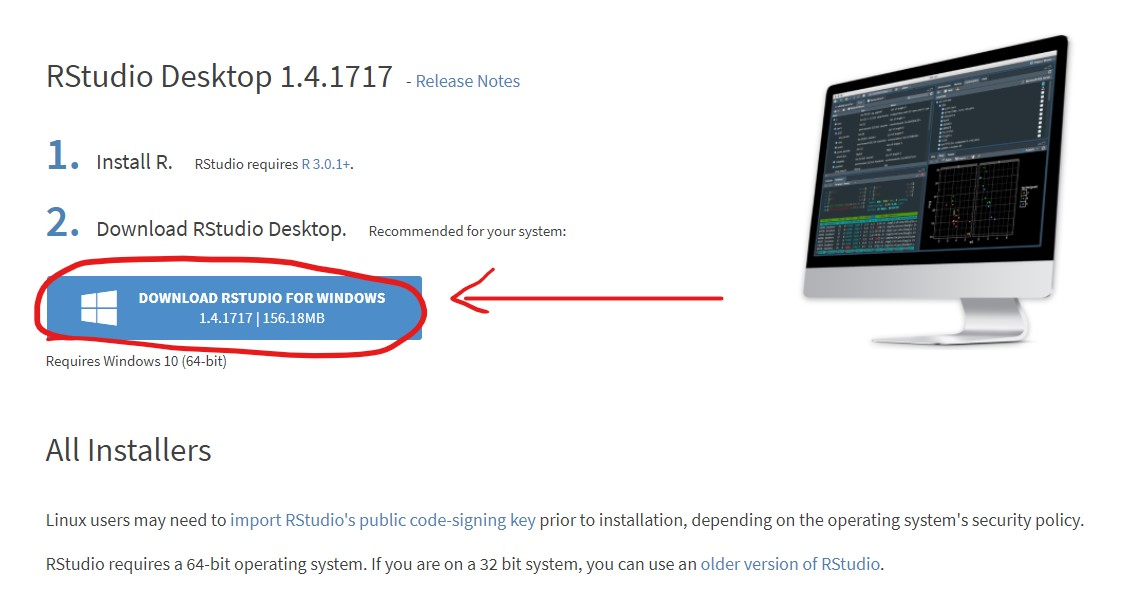
\includegraphics[width=6.25in,height=\textheight]{images/installr3.jpg}}

If the installation process of R and RStudio is finished, then we can open RStudio and start to learn the software.

  \bibliography{references.bib}

\end{document}
